% !TeX root = ../../../main.tex
\begin{figure}[htbp]
\begin{ChSixFloatBody}

% \footnotesize
% \centering
% 
\begin{minipage}[t]{\dimexpr \textwidth\relax}\centering

  \begin{minipage}[t]{0.65\textwidth}\vspace{0pt}
      % Force top alignment
    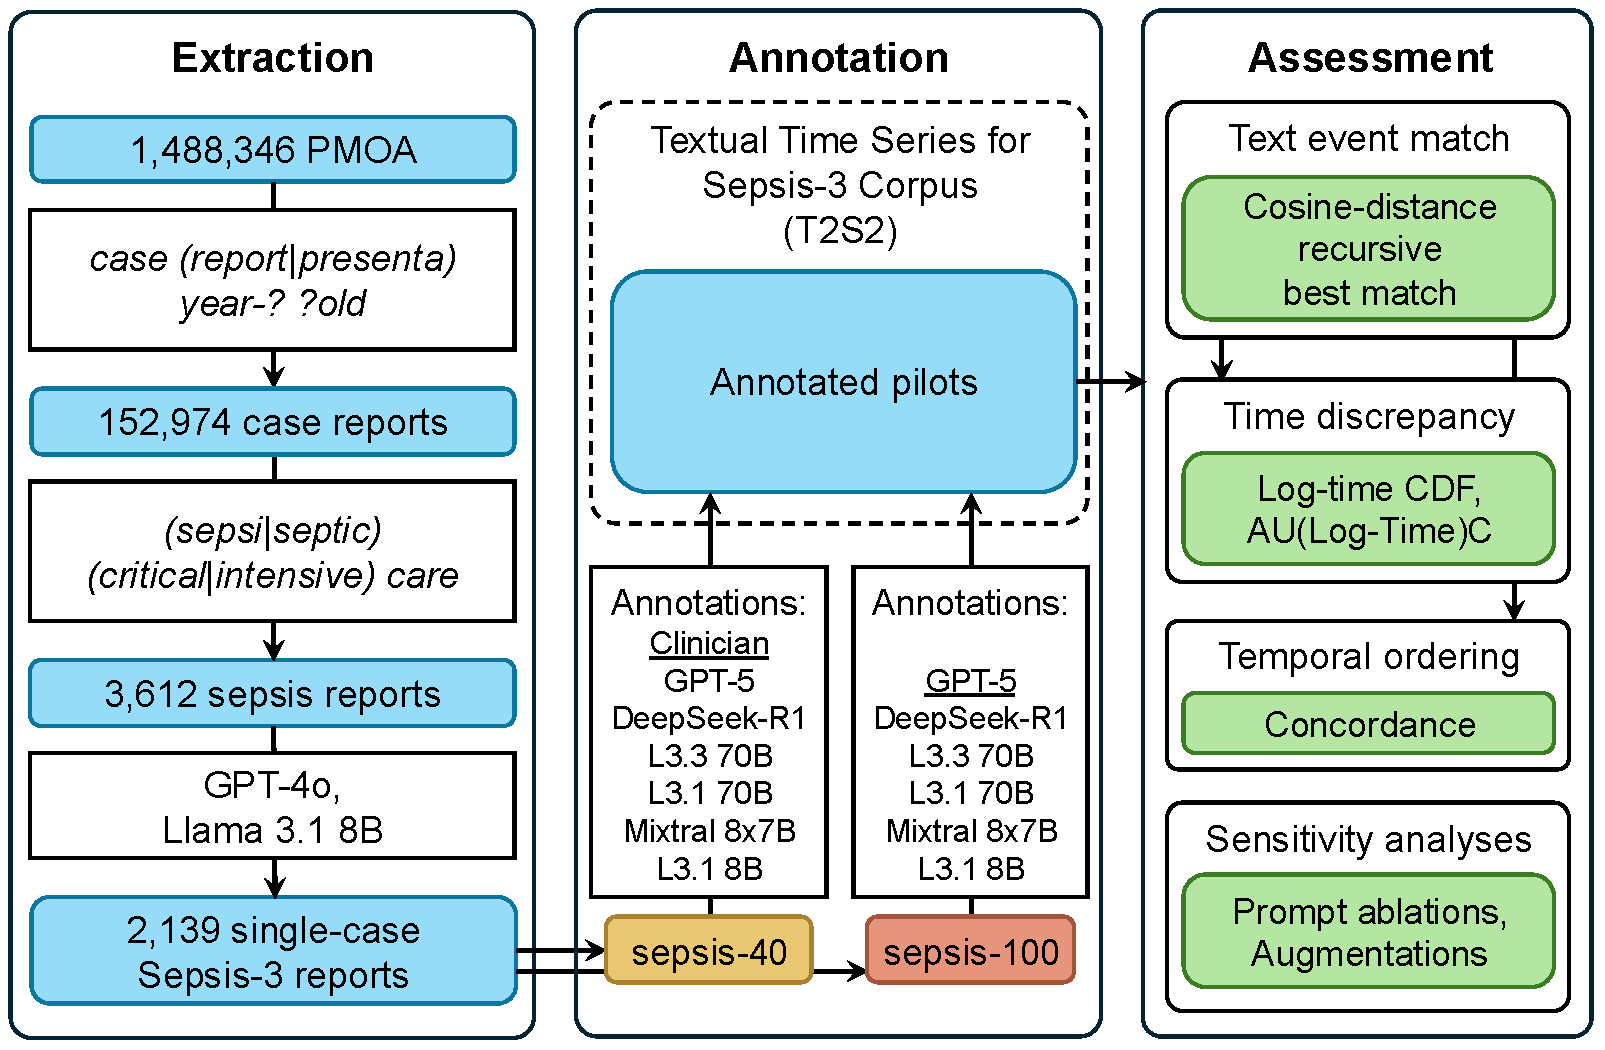
\includegraphics[width=\linewidth]{Chapters/chapter-06/images/figures/T2S2-CHIL-Main-Figure.pdf}
  \end{minipage}%
  % \hfill
  \hspace{.5em}
  \begin{minipage}[t]{0.30\textwidth}\vspace{0pt}
      % Force top alignment
    \begin{adjustbox}{max width=\linewidth}\begin{tabular}{r|cc}
    \multicolumn{3}{c}{\textbf{i2m4}} \\
    \midrule
    Qwen\textbackslash Human & Yes & No \\
    Yes & 2 & 0 \\
    No  & 0 & 18 \\
    \toprule
    L3.1 8B & Yes & No \\
    Yes & 2 & 7 \\
    No  & 0 & 11 \\
    \midrule
    \multicolumn{3}{c}{\textbf{\texttt{sepsis-100}}} \\
    \toprule
    GPT-4o\textbackslash Qwen & Yes & No \\
    Yes & 78 & 7 \\
    No  & 8 & 7 \\
    \toprule
    L3.1 8B & Yes & No \\
    Yes & 81 & 12 \\
    No  & 5 & 2 \\
    \bottomrule
    \end{tabular}\end{adjustbox}
  \end{minipage}

  
  
  
  
\end{minipage}

\end{ChSixFloatBody}
\caption{Flowchart of the PMOA T2S2 corpus construction pipeline (left).
    Confusion matrices (right) for Sepsis-3 phenotype in i2m4 (top) and \texttt{sepsis-100} (bottom) datasets, with preferred annotator in column position.}\ChSixFloatLabel{ch06:fig:flow}
\end{figure}